\documentclass{article}
\usepackage{graphicx}
\usepackage{algpseudocodex}
\usepackage{amsmath}
\usepackage{amssymb}
\usepackage{listings}
\usepackage{color}

\renewcommand{\ttdefault}{pcr}
\lstset{ 
    basicstyle=\color{black}\ttfamily,
    keywordstyle=\color{purple}\bfseries,
    commentstyle=\color{gray},
    numberstyle=\color{lightgray},
    stringstyle=\color{blue},
    identifierstyle=\color{brown},
    % escapeinside={\`}{\`},
    breakatwhitespace=false,
    breaklines=true,
    extendedchars=true,
    keepspaces=true,
    numbers=left,
    showspaces=false,
    showstringspaces=false,
    showtabs=false,
    tabsize=8,
    title=\lstname,
}
\lstdefinelanguage{JavaScript}{
  keywords={break, case, catch, continue, debugger, default, delete, do, else, false, finally, for, function, if, in, instanceof, new, null, return, switch, this, throw, true, try, typeof, var, void, while, with},
  morecomment=[l]{//},
  morecomment=[s]{/*}{*/},
  morestring=[b]',
  morestring=[b]",
  morestring=[b]`,
  ndkeywords={class, export, boolean, throw, implements, import, this},
  keywordstyle=\color{blue}\bfseries,
  ndkeywordstyle=\color{darkgray}\bfseries,
  identifierstyle=\color{black},
  commentstyle=\color{purple}\ttfamily,
  stringstyle=\color{red}\ttfamily,
  sensitive=true
}

\title{Crazy Quines}
\author{Maxwell Tang}
\date{Due 10 May 2024}

\begin{document}
\maketitle
Okay, so we've just received our first message from the great unknown,
    and it looks like the strangers from another world have another world have something to share with us!
After decoding the message we wait to see what it is. \vspace*{0.25cm}
\\Maybe it's a polynomial time solution for 3-SAT.
\\Maybe it's a proof of the Goldbach conjecture.
\\Maybe it's a computer virus that destroys our planet.
\bigbreak
It's a TypeScript interpreter.
\bigbreak
Well this is certainly unexpected, but regardless, we still need to come up with a response.
If first encounters here on earth have taught us anything,
    then we should realize that they're probably not just looking for friends,
    so it would be prudent to show that we're not just an empty planet full of free resources.

To do this, we can send a computer program back to them,
    and since they sent us a Typescript runtime,
    it would be natural to send a Typescript program back.
We don't know what kinds of programs would be interesting to them,
    but quines seem like a good candidate for a "universally interesting" program.

The problem is, though, that these guys are thousands of light-years away!
There's no way that our signal is getting to them intact.
What we need is a quine that can survive being corrupted.
In particular, a quine that prints its original output after a single character deletion would be a good starting point.
With a goal in mind, let's start working on it!

\subsection*{Existing Radiation-Proof Quines}
To begin, it makes sense to look at existing samples of radiation-proof quines in other languages.
In particular, an example from the Code Golf Stack Exchange is relatively easy to understand.
\lstinputlisting[language=JavaScript]{SEQuine.js}
As explained in the post, the script begins with a "guard statement" that accounts for typos created by the irradiation process.
This effectively "disables" any typos, and also absorbs any changes within itself.
Getting this part to work correctly relies on some JavaScript-specific features, so this likely won't be of much help to us.
The next part contains a repeated setTimeout statement, which both execute the quine-printing code.
The key in this part is that each statement only prints the quine if a certain flag has not been set.
This way, the second block acts as a backup incase the first block fails due to a missing character.

Unfortunately, because of how TypeScript works, every valid script must start with a keyword such as \verb|const|, \verb|let|, \verb|function|, etc.
Since the keywords in TypeScript are not lexically close enough to allow for clever tricks, any script can be made invalid by changing the first keyword.
Indeed, similar reasoning shows that most languages, like C, C++, Rust, Java, etc. have keywords as their Achilles' heels.
This, however, shouldn't lead us to lose hope.
We can loosen our requirements and see what cen be done.
For a start, we can still use the tricks outlined above to make our script valid under \textit{most} deletions, so that we will still probably get our message across.
In addition, we should also make sure that the script doesn't output the wrong text. We just want it to crash if it isn't able to print itself.
Finally, we might want to avoid manually crashing the program, since this might confuse the aliens into thinking that out quine is supposed to crash!

To begin, we can try making a basic quine in TypeScript(See quine.ts).
This follows the strategy listed out in David Madore's article on quines:
It begins with a data section,
    listing out most of the source code in the quine,
    followed by code to translate this into the actual source code fo the quine and printing it out.

This is a good first step, but we haven't actually done any radiation-proofing to this quine.
Indeed, when we run it through a testing script, we get 445 mutants which output the wrong text.










\section*{Examples!}

\subsection*{Equations}
$$\int_{0}^{\pi}\sin x dx = 2$$

\subsection*{Diagrams}
\begin{center}
    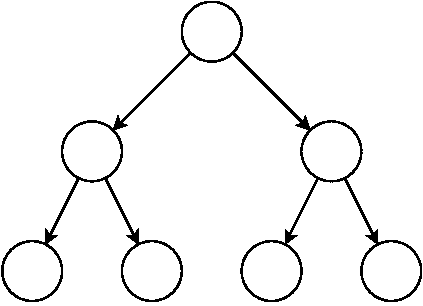
\includegraphics[width=0.5\textwidth]{example-figure.pdf}
\end{center}

\subsection*{Algorithms}
\begin{algorithmic}
    \Function{factorial}{n}
        \State x := 1
        \ForAll{i from 1 to n}
            \State x := x * i
        \EndFor
        \State \Return x
    \EndFunction
\end{algorithmic}

\subsection*{Code}
\lstinputlisting[language=C]{example-code.c}
\end{document}
